\documentclass[]{article}

%opening
\usepackage{amsmath,amssymb,amsfonts,amsthm,braket,cancel}
\usepackage{listings,xcolor,enumitem,tikz,physics,pgfplots}
\usetikzlibrary{calc,decorations.markings,positioning}
\usepackage[margin=1.0in]{geometry}
\usepackage{bbold}
\newcommand*{\QED}{\null\nobreak\hfill\ensuremath{\blacksquare}}
\numberwithin{equation}{section}
\usepackage{xurl,algorithm,algpseudocode}
\usepackage{fancyhdr,pdfpages}
\usepackage{bytefield,pgf-umlsd,svg}

\setlength{\parindent}{0em}

\newcommand{\newthreadShift}[4][gray!30]{
  \newinst[#4]{#2}{#3}
  \stepcounter{threadnum}
  \node[below of=inst\theinstnum,node distance=0.8cm] (thread\thethreadnum) {};
  \tikzstyle{threadcolor\thethreadnum}=[fill=#1]
  \tikzstyle{instcolor#2}=[fill=#1]
}

\lstset{ %
	language=sh,                     % the language of the code
	basicstyle=\footnotesize,       % the size of the fonts that are used for the code
	numbers=left,                   % where to put the line-numbers
	numberstyle=\tiny\color{gray},  % the style that is used for the line-numbers
	stepnumber=1,                   % the step between two line-numbers. If it's 1, each line
	% will be numbered
	numbersep=5pt,                  % how far the line-numbers are from the code
	backgroundcolor=\color{white},  % choose the background color. You must add \usepackage{color}
	showspaces=false,               % show spaces adding particular underscores
	showstringspaces=false,         % underline spaces within strings
	showtabs=false,                 % show tabs within strings adding particular underscores
	frame=single,                   % adds a frame around the code
	rulecolor=\color{black},        % if not set, the frame-color may be changed on line-breaks within not-black text (e.g. commens (green here))
	tabsize=2,                      % sets default tabsize to 2 spaces
	captionpos=b,                   % sets the caption-position to bottom
	breaklines=true,                % sets automatic line breaking
	breakatwhitespace=false,        % sets if automatic breaks should only happen at whitespace
	title=\lstname,                 % show the filename of files included with \lstinputlisting;
	% also try caption instead of title
	keywordstyle=\color{blue},      % keyword style
	stringstyle=\color{teal},      % string literal style
	escapeinside={\%*}{*)},         % if you want to add a comment within your code
	morekeywords={*,...}            % if you want to add more keywords to the set
} 

%\begin{figure}[h]
%    \centering
%    \includegraphics[scale=0.35]{.png}
%    \caption{}
%\end{figure}

\renewcommand{\arraystretch}{1.5}

\begin{document}

\pagestyle{fancy}
\fancyhead[L]{Team 57}
\fancyhead[C]{COMP90024 - Assignment 2}
\fancyhead[R]{5 May 2025}

Team 57.
Team Members: Josh Childs (1549150), Enzo Noel (1675346), Molly Stow (1356089), YU-WEI LIN (1537312)

\section*{System Architecture}

\subsection*{Overview}
The system is designed to gather data from three different platforms: Bluesky, OpenAustralia and Reddit.
The data is then processed and stored in elastic search indexs, which can be queried by the user.
The system is designed to be modular and scalable, so that we can easily add new platforms or data sources in the future and handle varying amounts of data.


\subsection*{Bluesky}

Bluesky has a firehose which gives access to all changes on the bluesky network.
We open a websocket to the firehose endpoint \texttt{com.atproto.sync.subscribeRepos}.
When we receive a \texttt{RepoCommit}, we call the fission function \texttt{processPost} which handles decoding the message.
A commit could be a like on a post, a new post, a repost, or some other type of update.
\texttt{processPost} returns either a 200 with a JSON of the post which contains the \texttt{cid}, \texttt{did}, \texttt{text} and \texttt{createdAt} fields, or a 404 if the commit was not a post.
Bluesky uses \texttt{cid} as the unique identifier of a commit, so we reuse this in the elastic search index.
\texttt{did} is an identifier for the author of the post, \texttt{text} is the body of the post and \texttt{createdAt} is the post timestamp.

\subsection*{Open Australia}
The OpenAustralia (OA) API provide a REST API which we can use to query the Australian parliament's Hansard reports, and also some user comments.

A redis message queue is used to handle the data inflow from the OpenAustralia API.\
The queues are created by sending a post request to the \texttt{enqueue} function, which allows messages to be stored in ``topic'' queues. 

The general structure of the OpenAustralia data inflow is as follows:
\begin{enumerate}
    \item An ``entrypoint`` fission function is called, which adds the parameters (keys) of the request to the redis message ueue \texttt{oa\_debate\_keys}.
    
    \begin{lstlisting}[frame=none,numbers=none]
    { 
        "house": "senate" or "representatives",
        "date" or "person": date in format YYYY-MM-DD or person id
    }
    \end{lstlisting}


    \item The \texttt{oa-debate-harvester-by-details} fission function is triggered by this redis message queue. 
    
    This function queries the OpenAustralia API for the debate details, and then queries the OpenAustralia API for the comments on that debate. This raw data is then stored in another redis queue \texttt{oa\_debates\_data}.
    \item The \texttt{debate-adder} fission function is triggered by this redis message queue. 
    The data is then processed and stored in the elastic search index \texttt{oa-debates-comments}.
    
    A parent-child relationship is created between the debate and the comments, so that we can query the comments for a specific debate.
    And also between debates and their parent topics, so that we can query the debates for a specific topic.
\end{enumerate}


There are three main entrypoints to gathering OpenAustralia data.

\begin{itemize}
    \item \texttt{oa-date-lister} - Queries the OpenAustralia API for dates in a year where debates were held.

    This uses a httptrigger route \texttt{oa-dates-with-debates}, providing the year as a parameter.

    \item \texttt{oa-person-lister} - Queries the OpenAustralia API for all debates held by a specific person.
    
    This uses a httptrigger route \texttt{oa-people-year-house}, providing the year and house (senate or represenatives) as parameters.

    \item \texttt{oa-daily-debate-harvester} - Queries the OpenAustralia API for all debates held on a specific date, and then queues the results for processing.
    
    This is accessed through a time trigger, which runs once a day.
\end{itemize}
The first two entrypoints are called manually to scrape past data from the backlog, while the third is called daily to gather new data.

All of the functions needed to gather and process OpenAustralia data are contained within the \texttt{oa-debates} fission package.

\subsection{Reddit Data Processing Architecture} 

The architecture for harvesting and processing data from Reddit is designed to accommodate both ad-hoc, parameterized data scraping and automated daily collection of recent posts. This system utilizes a Fission serverless workflow, orchestrated with Redis message queues, to efficiently manage the data flow from the Reddit API to Elasticsearch.

The Reddit data pipeline consists of the following key Fission functions and components:

\begin{enumerate}
    \item \textbf{Entrypoint Functions (Initiating Data Collection):} 
    There are two primary Fission functions that serve as entrypoints for Reddit data collection:

    \begin{itemize}
        \item \textbf{HTTP Triggered Harvester (\texttt{reddit-harvester-new-r}):}
            This function is invoked via an HTTP POST request to the \texttt{/reddit-new/scrape/} route.
            It is defined by the \texttt{reddit\_harvester.py:main} entrypoint.
            The function expects a JSON payload specifying:
            \begin{itemize}
                \item \texttt{keywords}: A list of keywords to search for.
                \item \texttt{subreddits}: A list of subreddit names.
                \item \texttt{limit} (optional, default: 10): The maximum number of posts to retrieve per keyword/subreddit.
                \item \texttt{scrape\_from} (optional, default: "2000-01-01"): A start date (YYYY-MM-DD format) for fetching posts created after this date.
                \item \texttt{scrape\_until} (optional, default: current date): An end date (YYYY-MM-DD format) for fetching posts created up to this date.
                \item \texttt{sort} (optional): The sorting method for Reddit search results (e.g., "new", "top", "relevance").
            \end{itemize}
            Upon receiving a request, \texttt{reddit\_harvester.py} uses the PRAW library to query the Reddit API for posts matching these criteria. It also extracts top-level comments for each retrieved post using the \texttt{get\_post\_comments} helper function within the script.
            The collected posts and their associated comments are formatted into JSON objects. These JSON objects (representing a list of posts/comments) are then enqueued into a Redis message queue named \texttt{reddit\_posts\_queue}. This enqueueing operation is handled by the \texttt{util.py:enqueue\_data} function, which makes an HTTP POST request to a generic Fission \texttt{enqueue} function.

        \item \textbf{Timer Triggered Daily Harvester (\texttt{reddit-daily-job}):}
            This function is automatically executed once a day, triggered by a Fission timer configured with a \texttt{@daily} cron schedule.
            It executes the \texttt{reddit\_daily\_harvester.py:main} entrypoint.
            The script queries the Reddit API for posts based on a predefined list of subreddits (\texttt{DAILY\_SUBREDDITS}) and keywords (\texttt{DAILY\_KEYWORDS}) hardcoded within the script.
            It focuses on posts created within a specific recent period defined by \texttt{DAILY\_SCRAPE\_DAYS\_AGO} (e.g., 1 day by default, but configurable as per the script's constants). The \texttt{DAILY\_LIMIT\_PER\_KEYWORD\_SUBREDDIT} and \texttt{DAILY\_SORT\_METHOD} are also configurable constants.
            Similar to the HTTP harvester, this function gathers posts (and can be configured to gather their top-level comments via \texttt{get\_post\_comments\_for\_daily}). The formatted JSON data is enqueued into the same \textbf{\texttt{reddit\_posts\_queue}} using \texttt{util.py:enqueue\_data}.
            The hardcoding of subreddits and keywords in the daily harvester is a deliberate choice to simplify automated daily scraping; these parameters could ideally be externalized to the \texttt{shared-data} ConfigMap for greater flexibility.
    \end{itemize}

    \item \textbf{Data Queuing (Redis):} 
    Both harvester functions send their collected and formatted data (as JSON strings, typically representing batches of posts/comments) to a central Redis list acting as a message queue, named \textbf{\texttt{reddit\_posts\_queue}}.
    The address for the Redis instance used by the Fission Message Queue Triggers is \texttt{redis-headless.redis.svc.cluster.local:6379}.

    \item \textbf{Data Indexing into Elasticsearch (Adder Function):}
    The \textbf{\texttt{reddit-to-es-new-r}} Fission function, with its entrypoint at \texttt{reddit\_to\_elasticsearch.py:main}, is responsible for consuming data from the \texttt{reddit\_posts\_queue}.
    It is triggered by a Fission Message Queue Trigger (MQT) of \texttt{mqtkind keda}, which monitors the \texttt{reddit\_posts\_queue}.
    When new messages (batches of posts/comments) arrive, KEDA invokes \texttt{reddit-to-es-new-r}.
    The function iterates through each post or comment in the received batch.
    For each item, it checks if a document with the same \texttt{post\_id} (which serves as the unique identifier for both posts and comments) already exists in the Elasticsearch index named \textbf{\texttt{reddit}}. This check prevents duplicate entries.
    If the item does not exist, it is indexed into the \texttt{reddit} index. The mapping for this index is defined in \texttt{reddit-index.json}.
    If message processing fails after the configured number of retries (e.g., 3 retries), the problematic message is moved to an error topic/list in Redis named \texttt{reddit\_adder\_error} for later analysis and debugging.
\end{enumerate}

This multi-stage, queue-based architecture allows for decoupling of data harvesting and data indexing, providing resilience and scalability. All Fission functions related to the Reddit pipeline are part of the \texttt{reddit-harvester-new-r} Fission package and utilize the \texttt{shared-data} ConfigMap for configurations such as API keys and Elasticsearch connection details.


\subsection*{Sentiment Analysis}

\paragraph*{Choosing an Analysis Method}
In order for us to perform sentiment analysis on the posts from the various social media platforms we whose, we had to choose between different avaiable options. However, since we didn't want to reinvent the wheel and risk having analysis of lesser quality we decided to use a pre-existing library. Now the choice of library came down to ease of use and overall consistency with our project.

This is why we decided to use the \texttt{VADER} library. VADER is a lexicon and rule-based sentiment analysis tool that is specifically tuned to sentiment analysis in social media posts and text. It is capable of detecting sentiment in text, and it is particularly effective for short texts such as tweets or posts.

\paragraph*{Putting it into Practice}
For our project, we decided to keep the sentiment analysis simple and only use a couple of values from the vader sentiment analysis function which are the following: positive, negative and neutral.

The next step was of course to implement the analysis function in our code and make it available for other functions to use. This was done by creating a new fission function called \texttt{sentiment-analysis} which takes in a string and returns the sentiment analysis values. We had to manage the dependencies and make sure that the fission function had access to the \texttt{VADER} library. This was done by creating a fission package.

\subsection*{Named Entity Analysis}

\subsection*{Analysis}

Performing the analysis described above takes a non trivial amount of time. 
3 simple options come to mind to handle this.

\begin{itemize}
    \item Calculating the analysis results for all posts. 
        Given the large number of posts we have in some indexes, bluesky in particular, this would be infeasible.
    \item Run the analysis on the posts queried by the user. 
        This may take a long time if the query contains a large number of posts.
    \item Setup a fission function to periodically calculate and store the values for a subset of posts.
        This would be a better option than the two previous ones, but requires foresight into what posts are relevant, or increased effort in changing the focus.
\end{itemize}

Given the disadvantages of each, instead we implement a hybrid of 2 and 3.
We calculate the values for posts queried by the user, and cache these in a separate elastic search index. 
When the user queries those posts again, we pull values from the cache index instead of using the analysis functions.
This process is described in Algorithm~\ref{alg:cap}.
To increase throughput, we send the cache function a list of post id's to retrieve, reducing the overhead of authenticating elastic search clients.

\begin{algorithm}
    \caption{Caching Analysis Results}\label{alg:cap}
    \begin{algorithmic}
        \State $ \texttt{Ids} \gets [id_0, \dots, id_n] $ 
        \State $ \texttt{Index} \gets index $ \Comment{ElasticSearch index containing the id's}
        \State $ \texttt{Field} \gets field $ \Comment{Field which is being analysised}

        \State $ \texttt{CacheEntry} \gets \texttt{queryESForIds}(\texttt{Ids}, cacheName, \texttt{Index}) $ \Comment{\parbox[t]{.4\linewidth}{Fetch any entries from the elastic search cache index which match the index and any id in Ids}}

        \For{$ id $ in $ \texttt{Ids} $}
            \If{$id$ not in $ \texttt{CacheEntry} $}
                \State $ text \gets \texttt{queryES}(\texttt{Index}, id, \texttt{Field}) $ 
                    \Comment{\parbox[t]{.4\linewidth}{Query \texttt{Index} for the document with id 
                    \texttt{id} and retrieve the field \texttt{Field}}}
                \State $ value \gets \texttt{queryAnalysisFunction}(text) $ 
                    \Comment{Compute the value to cache}
                \State \Call{insertES}{cacheName, \texttt{Index}, id, value} 
                    \Comment{Insert the value to the cache index}
                \State \Call{append}{\texttt{CacheEntry}, \{id, value\}}
            \EndIf
        \EndFor

        \State \Return $ \texttt{CacheEntry} $
    \end{algorithmic}
\end{algorithm}

\subsection*{User Interface}

\section*{Scenarios}

\paragraph*{Overview}
Today, it is nearly impossible to spend time online without witnessing a discussion about politics. For many people, this is not a topic that is discussed politely, calmly and with respect. A thread on a hot topic quickly can become intense, escalating into arguments and attacks. 

But is it truly like this everywhere, or are we just seeing the worst side of the internet? 

Are there still sides of social media where people present their political opinions in a pleasant and happy way? 
And where does all this anger come from? 
Are Australians egged on by high valence political speeches? Do some politicians and parties use more aggressive language, and does this align with the discussions they spark? 


In this project, we set out to answer these questions by analysing political discussions held on two different platforms: Bluesky and Reddit.
We thought it would be interesting to compare the sentiment and topic of these discussions to those of political speeches being held in parliament, as provided through OpenAustralia.

\subsection*{Analysis Goals}
We had three main goals for our analysis.

\paragraph*{Comparing the topics}
We first wanted to see what political topics were popular for discussion across platforms. 
Do users of different social media platforms have different priorities? Do they discuss the same topics, and do these align with what is being discussed in parliament?
We investigated topics such as “housing”, and entities, including politicians such as “Pauline Hansen”, Australian locations, and parties, such as "Labor".

\paragraph*{Comparing the overall sentiment}
We aimed to contrast the overall sentiment of these discussions and debates over time.
We wanted to see if the conversations held on some of these platforms were more positive or negative than others, and whether there were any clear trends.

\paragraph*{Comparing the sentiment by topic}
We also wanted to see if the sentiment of these discussions differed depending on the topic being discussed.
For example, do users of Reddit post more positively about the topic of housing than those on BlueSky?

\paragraph*{Comparing the topics over time}
We then wanted to contrast the sentiment and topics of these social media discussions to the actual debates being held. 
This allowed us to see if topics were discussed immediately after a relevant debate, and whether an intense debate correlated with a shift in sentiment online.


\subsection*{Fission}

\subsection*{Fission Specs}
In alignment with the principle of declarative application management, we used fission specs to define the desired state of our fission setup. 

This allows us to easily manage the state of our system, add new functions and edit the configuration of existing functions.
It also means that our infastructure is ``self healing'', as fission will automatically re-deploy any functions which are not in the desired state.
This was espeically important when working in a shared environment with a large number of group members.


\section*{NeCTAR Research Cloud}

\subsection*{Platform Discussion}

\subsection*{Challenges (we can remove this, its just mentioned that we should talk about challenges)}
A major challenge our group faced was adapting to the shared nature of the NeCTAR research cloud.
At several points during the project, we encountered issues arising from multiple people attempting to modify the system at once.

These were generally minor, such as applying conflicting fission specs.
However, we also encountered more serious issues.
Near the beginning of the project, the cluster setup was unexpectedly re-run, meaning that we had to re-build our software stack.

Even at a small group scale, it was difficult to coordinate the changes being made to the system.

This was somewhat mitigated by the use of fission specs, as we could easily re-deploy the functions to a different worker node.
These challenges highlighted the benefits of using an Infrastructure as Code approach, as we could recover from these setbacks.

\subsection*{Application Scaling}

\paragraph*{Bluesky} To handle processing the large number of posts in the bluesky firehose, we utilise a new deploy pool of fission functions.
We set the minimum number of pods to 1, and the maximum to 30. 
This allows fission to increase or decrease the number of pods, up to 30, depending on the current load.

\paragraph*{OpenAustralia} 
The data influx of the OpenAustralia api was of a less intense ``velocity'' compared to that of BlueSky and Reddit.
This meant that the regular scraping could be done on a daily basis, gathering data from debates held two days prior, with to allow complete collection of data, as the Hansard reports are finalised by 5pm the day after the debate.
This was achieved using a time based fission trigger \texttt{oa-daily-debate-harvester}, which runs once a day.
Similarly to the BlueSky setup, the number of pods were dynamically allocated as needed. However, due to the lower amount of incoming data the minimum number of pods was set to 0, as the resources required when starting a new pod would not significantly affect the performance.
\\
The message queues used a Keda workload autoscaler.
This monitored the number of messages in the queue, and scaled the number of pods up or down depending on the number of pods required.
This helped handle the variabible load of the OpenAustralia API, as the number of messages in the queue could vary from 0 to 1000+, especially when gathering data from previous years. 

As a side comment, the usefulness of the \texttt{oa-daily-debate-harvester} was limited while collecting data for our project, as The Houses of Parliament are in recess from 16 May until 25 May 2025 and so no new debates were available to add.


\subsection*{Error Handling}

\paragraph*{Bluesky} The bluesky websocket runs inside a container, instead of a fission function, since the websocket can listen indefinitely.
This container is deployed to kubernetes with one replica. 
This means the container will be re-deployed to another worker node if one fails, and kubernetes will spin up another replica if the current one crashes from an error.


\paragraph*{OpenAustralia} 
A modular, ``Event Driven Architecture'' approach was taken to handle errors in the OpenAustralia API.\ 
The logic associated with querying the OpenAustralia API was split into three key parts: the entrypoint functions, the harvester, and the adder.

These are connected by redis message queues, each with their own ``error topics''.
This seperation of functionality improves the robustness of the system, as we can see exactly where any errors occurred, and retry only that part of the process. Somethiungsomething Event driven architecture
\
It also means that if one part of the process fails, the outputs of the other functions will still be saved, allowing the process to continue without data loss.

This was particularly useful when querying the OpenAustralia API, as the formatting of responses is often unpredictable, even within the same endpoints.
\\
The immediate httptrigger entrypoint functions do not have any retry logic, as they are only called once manually, and the data is stored in the redis queue.
The \texttt{oa-debate-harvester-by-details} and \texttt{debate-adder} functions are triggered by the redis queues, and have retry logic built in. 
Both of these functions will retry up to 3 times if they encounter an error, and will log the error message to their respective ``error topic'' redis queue.
\\
This strategy is certainly not perfect, as it does not handle all possible errors, but it does allow us to see where the errors are occurring, and retry the failed functions.

\paragraph*{Reddit}
Similarly to the OpenAustralia API, the reddit harvester is split into three parts: the entrypoint, the harvester and the adder. 
This provided all the same benefits as the OpenAustralia API, including seperation of functionality, and the ability to retry failed function and greater insight into where errors are occuring.


\subsection*{Integration Testing}



\subsection*{Analysis}


\subsubsection*{Comparing the topics: Topic visualisation through word clouds}

\begin{figure}[h]
    \centering
    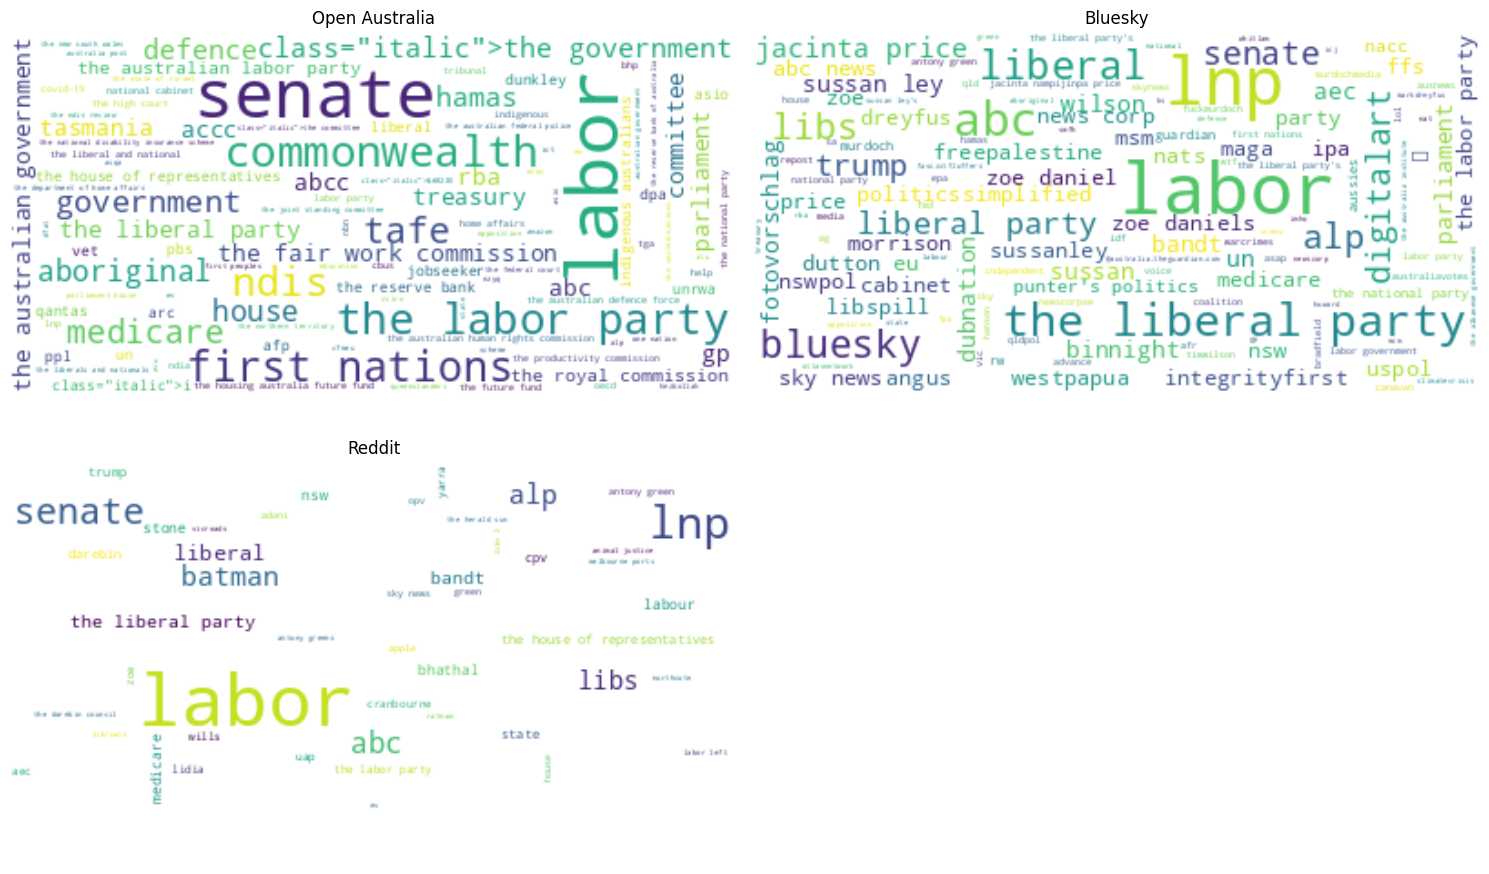
\includegraphics[scale=0.35]{report_images/wordcloud-org.png}
    \caption{Word cloud of the most common ``Organisation'' entities in the posts and debates.}
\end{figure}

Whatever we found here. btw will replace with final images
To visually compare the topics of the posts and debates, we word clouds to show the most common entities in the posts and debates.
Analysis was performed using the \texttt{spacy} library, and the word cloud was generated using the \texttt{wordcloud} library.

\subsubsection*{Comparing the overall sentiment: Stacked bar chart over time}

\begin{figure}[h]
    \centering
    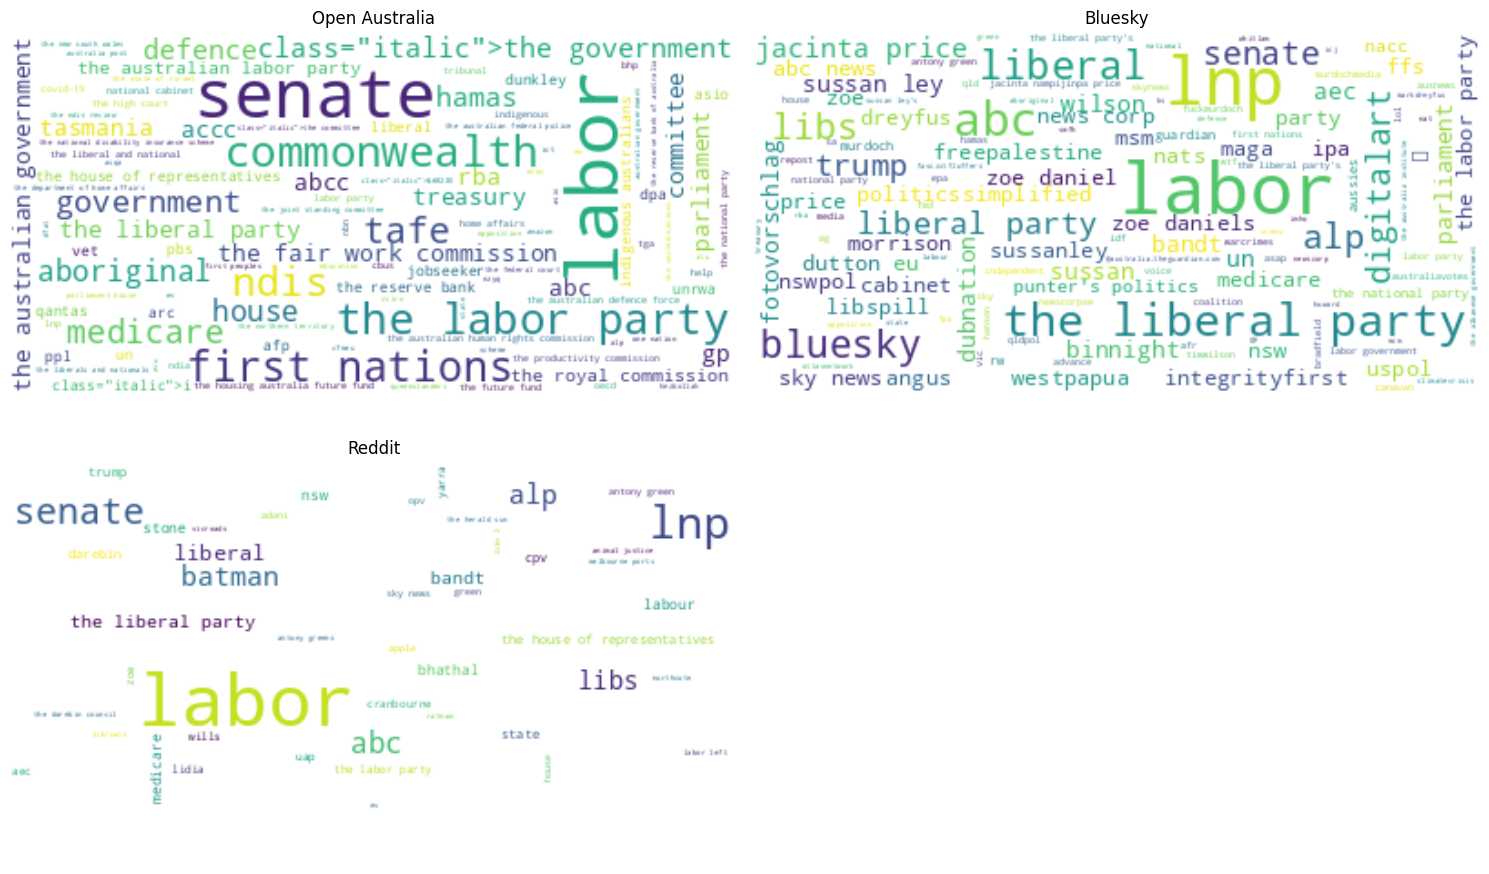
\includegraphics[scale=0.35]{report_images/wordcloud-org.png}
    \caption{Overall sentiment over time from TIME to TIME.}
\end{figure}
The overall sentiment of the posts and debates was calculated using the \texttt{VADER} library.
idk


\subsubsection*{Comparing the sentiment by keyword: idk what to call this one}
\begin{figure}[h]
    \centering
    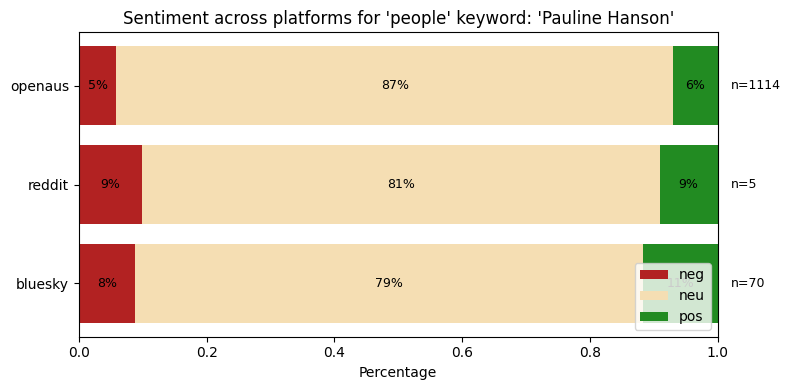
\includegraphics[scale=0.35]{report_images/sentiment-pauline.png}
    \caption{Comparison of sentiment for the keyword ``Pauline Hanson''.}
\end{figure}
A small number of topics were selected based on their prevalence in the posts and debates, and their relevance to the current political climate.

\subsubsection*{Comparing the topics over time: }

\begin{figure}[h]
    \centering
    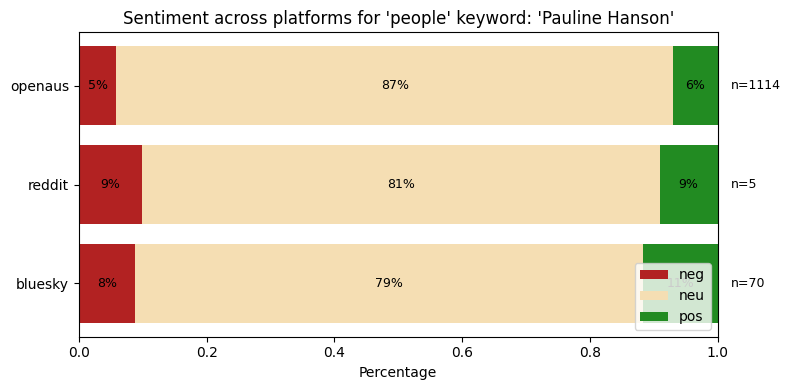
\includegraphics[scale=0.35]{report_images/sentiment-pauline.png}
    \caption{Comparison of sentiment for the keyword ``Pauline Hanson''.}
\end{figure}
idk need to fill in
\end{document}
